\documentclass[10pt]{article}
\usepackage{CJKutf8}
\usepackage{hyperref}
\usepackage{graphicx}
\usepackage{textgreek}

% can create colorful boxes, for warning p.ex.
\usepackage[most]{tcolorbox}

% making the text of the report sans serif
\renewcommand{\familydefault}{\sfdefault}

% solve the issue when there is a dollar sign
% in a listing. Uses $\dollar$ instead
\newcommand{\dollar}{\mbox{\textdollar}}

\title{Setting up and using micro-ROS the Nucleo-144 \\[1ex] \large \begin{CJK}{UTF8}{min}南山大学\end{CJK}}
\date{}
\author{Vincent Conus}

\begin{document}
 
\maketitle

\begin{figure}[h]
  \centering
  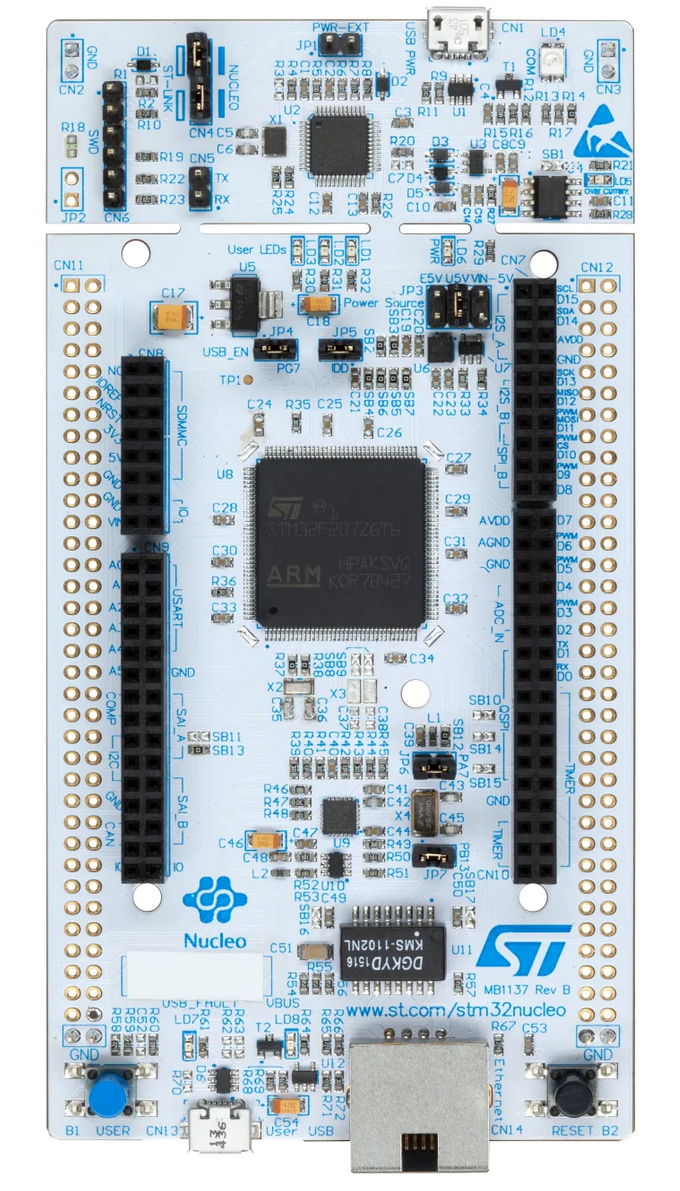
\includegraphics[width=0.5\textwidth]{./img/board.png}
\end{figure}

\pagebreak
\tableofcontents

\pagebreak
%--------------------------------------------------------------------------------------
\section{Introduction and motivation}
Being a widely available board from ST and with an official support for micro-ROS, the \href{https://www.st.com/en/evaluation-tools/nucleo-f429zi.html}{Nucleo-144} is a great board as an intermediate step on the journey to have a ROS2 ecosystem running on a system like the \href{https://gitlab.com/nitrogen8m/documentation}{Nitrogen8M} with an heterogeneous cores setup.\\
Running a micro-ROS instance on this board is a useful goal in the overall project, as it will
allow me to test the ``standard'' use-case of that technology.\\
Later on, the goal will be to be able to run the DDS system over RPMsg.\\

Note that throughout this guide, the board will be referred to as ``Nucleo'' or ``F7'', by the fact that it is based on a STM32F7* microcontroller\footnote{A very similar ``F4'' board was also tested, as presented in the appendix \ref{appendix:stm32f4}.}.

%--------------------------------------------------------------------------------------
\section{Blinking a LED}
\label{sec:blinking-led}
When working with a microcontroller, this is always the first step to be taken
in order to know that the board is working and that our toolchain is properly
configured to upload a firmware to the board.

\subsection{STM32CubeIDE}
\label{sec:stm32cubeide}
Similarly to what presented in \href{https://gitlab.com/stm32mp157f-dk2/documentation}{my documentation for the STM32MP157F board}, the current Nucleo board projects can also be edited and loaded through serial connection from the \href{https://www.st.com/en/development-tools/stm32cubeide.html}{STM32 Cube IDE}. This tool has the advantage of being directly provided by ST and having a lot of available functionality for building and debugging project, however, such project are extremely inconvenient to move and are close to impossible to port. Regardless, this is way we shall take for this guide, so as visible on the figure \ref{fig:ide} we are going to use the tool provided by ST to build and upload the firmware for our Nucleo board. The link in the previous paragraph explains how to install it.

\begin{figure}[h]
  \centering
  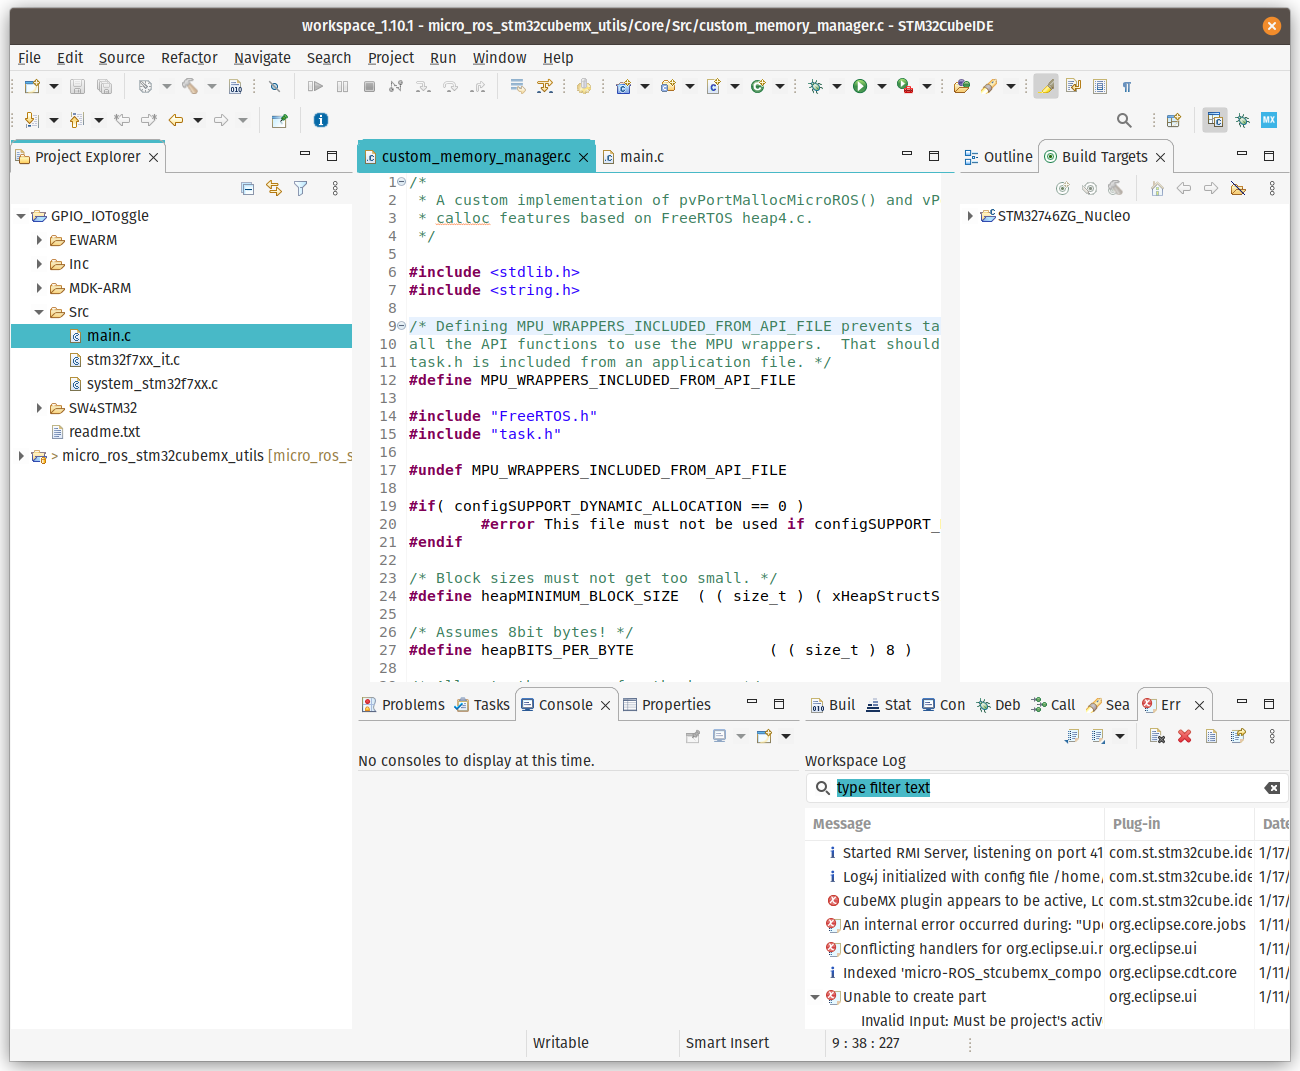
\includegraphics[width=0.85\textwidth]{./img/ide.png}
  \caption{The STM Cube IDE view, with a project opened}
  \label{fig:ide}
\end{figure}

\subsection{STM32F7 firmware package}
\label{sec:stm32f7-firmw-pack}
With the IDE ready to be used, we now have to get the firmware package for our board.
Since the Nucleo board we have is running a STM32F processor, we will need the similarly named pack.\\

The \href{https://www.st.com/content/st_com/en/products/embedded-software/mcu-mpu-embedded-software/stm32-embedded-software/stm32cube-mcu-mpu-packages/stm32cubef7.html}{STM32 cube F7 firmware package} is available at that link. Once the whole directory is download and decompressed, you can access all the template projects, navigating to the following directory (dependent on your actual version): \verb|./STM32Cube_FW_F7_vX.XX.X/Projects/STM32F746ZG-Nucleo/|. In particular, for our case as we want firstly to be able to blink an LED, we can navigate to further, into \verb|Examples/GPIO/GPIO_IOToggle|. This specific example is precisely what we want: a simple structure of a project that blinks the \verb|LED1| LED.

\subsection{Building and running the GPIO example}
\label{sec:build-runn-gpio}
The project downloaded as the F7 firmware, named \verb|GPIO_IOToggle| can be loaded into the IDE.
From the IDE interface, you can use \verb|File|, then \verb|Import...|, and then \verb|Existing Projects into Workspace|, as visible in the figure \ref{fig:import}. Then, as visible in the figure \ref{fig:project}, we can navigate to the \verb|GPIO_IOToggle| directory and open it as a project. You should have two nested project that can be imported here.

\begin{figure}[h]
  \centering
  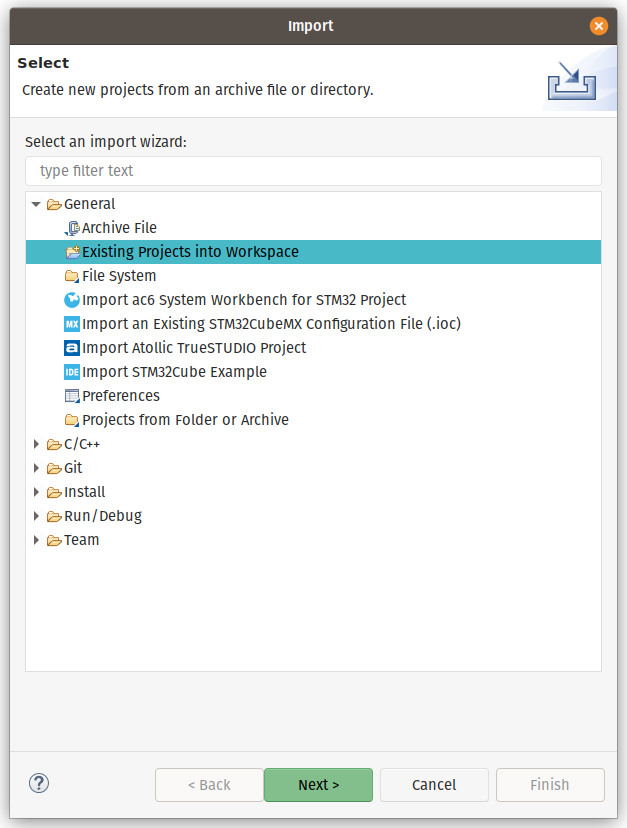
\includegraphics[width=.5\textwidth]{./img/import.png}
  \caption{Importing an existing project from the filesystem}
  \label{fig:import}
\end{figure}

\begin{figure}[!h]
  \centering
  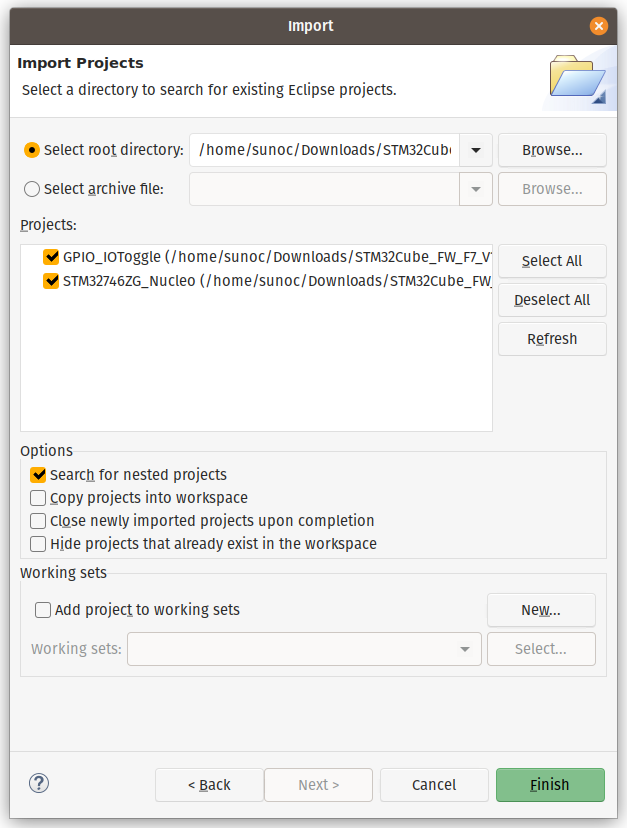
\includegraphics[width=.5\textwidth]{./img/project.png}
  \caption{Importing the nested GPIO projects}
  \label{fig:project}
\end{figure}

The project being imported, we can now see it's structure in the explorer of the IDE (figure \ref{fig:tree}). It also becomes clear here too why these STM Cube IDE are problematic to handle: even for such a simple task like the LED blink, a whole structure of inclusions and library that are elsewhere are needed.\\

However, with the Nucleo board plugged in the USB port of you computer, and by selecting the \verb|STM32746ZG| sub-project, you can build the example (hammer icon), and then run it (white arrow on a green dot icon).\\
As visible in the figure \ref{fig:toggle_led}, if you navigate around the line 90 of the \verb|main.c| file, you will find a delay function that takes some milliseconds in entry parameter. By changing that value, you are able to check if the code you are building is indeed being uploaded to the board.\\

With this setup, you should be able to build the example and having the LD1 LED on the top of your Nucleo board to blink.

\begin{figure}[h]
  \centering
  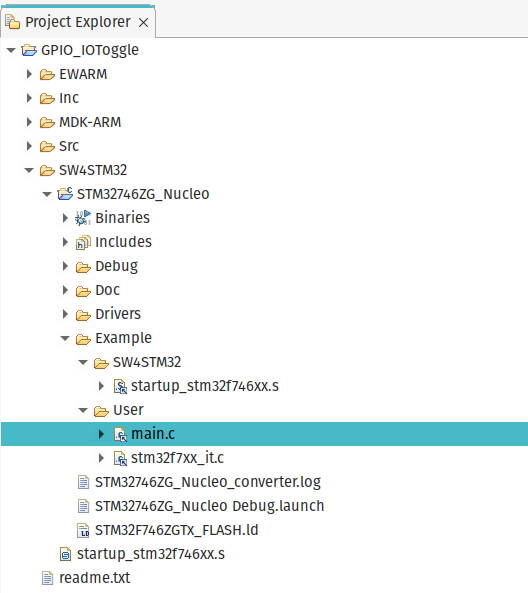
\includegraphics[width=.9\textwidth]{./img/tree.png}
  \caption{GPIO project structure}
  \label{fig:tree}
\end{figure}

\begin{figure}[!h]
  \centering
  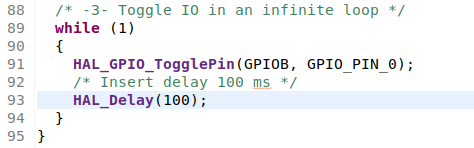
\includegraphics[width=.9\textwidth]{./img/toggle_led.png}
  \caption{``while'' loop with the toggling timing for the LD1 LED}
  \label{fig:toggle_led}
\end{figure}

\pagebreak
% --------------------------------------------------------------------------------------
\section{Setting up micro-ROS}
\label{sec:micro-ros}
Now we have a minimal project running on our Nucleo board, it's time to try, deploy and run a micro-ROS instance.
Deploying micro-ROS on a microcontroller is not a trivial task, as the firmware that is meant to be compiled and sent over must contain at least:
\begin{itemize}
\item The specific drivers for the board
\item A real-time operating system, most likely FreeRTOS
\item The micro-ROS layer itself
\item The program that will use this micro-ROS environment
\end{itemize}

Furthermore, it is every more hard to debug such deployment, since a micro-ROS is only visible as it communicates with a full-on ROS2 system.

\subsection{Local Linux micro-ROS running a ping-pong test app}
\label{sec:local-linux-micro}
The first step in the path of running micro-ROS, we should try to run a ping-pong application on my Linux machine.
Some instructions for this particular task are given on \href{https://micro.ros.org/docs/tutorials/core/first_application_linux/}{micro-ROS website}.
Alternatively, there is a \href{}{micro-ROS report prepared by Prof. Honda}, available in this very repository.\\

In this section of the report about the Nucleo board, I will present a tested, combined step-by-step guide on how to accomplish this task.\\

Docker is used in both guides to have a controlled environment to build and run these test tools.
It is then important to install it on your system (or even remotely). \href{https://docs.docker.com/engine/install/}{The official Docker documentation} is the way to go, and it depends on your operating system. Even on your desktop, the version you'd want is the ``server'' version, as it is more widely available and more lightweight. From here I will assume that you have a docker install handy.\\


The following commands will pull a ROS container, version \verb|foxy|, and name it \verb|ros_build|.
Then, we can execute \verb|bash|, as a way to open a terminal to the ``inside'' of the container.
\begin{tcolorbox}
\begin{verbatim}
sudo docker run -d --name ros_build -it --net=host -v \
     /dev:/dev --privileged ros:foxy
sudo docker exec -it ros_build bash
\end{verbatim}
\end{tcolorbox}


From inside the container, we can follow the micro-ROS wiki guide, as to have two micro-ROS nodes that can run a default ``ping-pong'' application, as a proof that the system works and that the instances are able to communicated with each other.\\
The following command list will pull the required firmware, build it, then build, setup and run the agents inside you Docker container:
\begin{tcolorbox}
\begin{verbatim}
. /opt/ros/$ROS_DISTRO/setup.bash

mkdir microros_ws
cd microros_ws
git clone -b $ROS_DISTRO \
    https://github.com/micro-ROS/micro_ros_setup.git \
    src/micro_ros_setup

sudo apt update && rosdep update
rosdep install --from-paths src --ignore-src -y
sudo apt-get -y install python3-pip wget nano

colcon build
. ./install/local_setup.bash

ros2 run micro_ros_setup create_firmware_ws.sh host

ros2 run micro_ros_setup build_firmware.sh
. ./install/local_setup.bash

ros2 run micro_ros_setup create_agent_ws.sh
ros2 run micro_ros_setup build_agent.sh
. ./install/local_setup.bash

ros2 run micro_ros_agent micro_ros_agent udp4 --port 8888
\end{verbatim}
\end{tcolorbox}

Once your agent is running, you can open another terminal in your Docker (similarly to what was presented above: \verb|sudo docker exec -it ros_build bash|), and run the following commands to start the micro-ROS pingpong app:
\begin{tcolorbox}
\begin{verbatim}
. /opt/ros/$ROS_DISTRO/setup.bash
. ./install/local_setup.bash

export RMW_IMPLEMENTATION=rmw_microxrcedds

ros2 run micro_ros_demos_rclc ping_pong
\end{verbatim}
\end{tcolorbox}

Then in yet another terminal, you can \verb|bash| into your container and run the following commands to actually test the running pingpong application:
\begin{tcolorbox}
\begin{verbatim}
. /opt/ros/$ROS_DISTRO/setup.bash

ros2 topic echo /microROS/ping
\end{verbatim}
\end{tcolorbox}

If you see some nanosec timestamp with a \verb|frame_id| value, you are doing it right !

\subsection{micro-ROS on a microcontroller}
\label{sec:micro-ros-micr}
Now we know that we can build micro-ROS agents, the goal is to build a firmware for our Nucleo board that can talk to our PC via serial.
This should be possible following the \href{https://micro.ros.org/docs/tutorials/core/first_application_rtos/freertos/}{official guide} since the board is \href{https://micro.ros.org/docs/overview/hardware/}{officially supported}.\\


Similarly to the previous section, we will \verb|bash| into our ROS2 Docker. From here, we can  pull the firmware for the STM32 boards and run the setup scrips, so from a fresh ROS2 Docker, you can run:
\begin{tcolorbox}
\begin{verbatim}
. /opt/ros/$ROS_DISTRO/setup.bash
mkdir microros_ws
cd microros_ws
git clone -b $ROS_DISTRO \
    https://github.com/micro-ROS/micro_ros_setup.git \
    src/micro_ros_setup

sudo apt update && rosdep update
rosdep install --from-paths src --ignore-src -y
sudo apt-get -y install python3-pip wget nano


ros2 run micro_ros_setup create_firmware_ws.sh \
freertos nucleo_f746zg

ros2 run micro_ros_setup configure_firmware.sh \
ping_pong --transport serial

ros2 run micro_ros_setup build_firmware.sh

ros2 run micro_ros_setup flash_firmware.sh
\end{verbatim}
\end{tcolorbox}
Note that it is possible to flash the binary directly, as shown in the appendix \ref{appendix:nucl-filesyst-from}.\\

We can then create the agent for the ROS2 that lives inside the container:
\begin{tcolorbox}
\begin{verbatim}
ros2 run micro_ros_setup create_agent_ws.sh
ros2 run micro_ros_setup build_agent.sh
. ./install/local_setup.bash
\end{verbatim}
\end{tcolorbox}

We have to get the local agent connecting to the topic, you can run (remotely, through the \verb|/dev/ttyACME0|) the firmware with the following command, and then plug-out and plug-in the usb cable:
\begin{tcolorbox}
\begin{verbatim}
ros2 run micro_ros_agent micro_ros_agent serial \
--dev /dev/ttyACM0
\end{verbatim}
\end{tcolorbox}
In some cases, if the agent does not return messages about subscribing to topics, unplugging and re-plugging is needed for the agent to be able to subscribe to the topic.\\

Finally, for testing this application, you can bash into the Docker from another term and run these:
\begin{tcolorbox}
\begin{verbatim}
. /opt/ros/$ROS_DISTRO/setup.bash

ros2 topic echo /microROS/ping
\end{verbatim}
\end{tcolorbox}
As stated in the official wiki: "At this point, we know that our micro-ROS app is publishing pings. ".\\

A slightly more complex setup is required to check the ``pong'', see if our micro-ROS app can receive and reply to messages.\\
Firstly, we will need three terminals with a bash session running in our Docker. As a reminder, this can be done as follow. You'll also need to have the \verb|setup.bash| in your path for each bash instance:
\begin{tcolorbox}
\begin{verbatim}
sudo docker exec -it ros_build bash
. /opt/ros/$ROS_DISTRO/setup.bash
\end{verbatim}
\end{tcolorbox}

Now, for each terminal opened.\\
You will need one that receive the pings form the Nucleo:
\begin{tcolorbox}
\begin{verbatim}
ros2 topic echo /microROS/ping
\end{verbatim}
\end{tcolorbox}

A second one that receive the pongs:
\begin{tcolorbox}
\begin{verbatim}
ros2 topic echo /microROS/pong
\end{verbatim}
\end{tcolorbox}

And the third one will publish fake pings, so the Nucleo board will reply with a ping:
\begin{tcolorbox}
\begin{verbatim}
ros2 topic pub --once /microROS/ping \
std_msgs/msg/Header '{frame_id: "fake_ping"}'
\end{verbatim}
\end{tcolorbox}

Running the command form the third term will show the fake ping in the second, but most critically, we will be able to see the pong, among the pings, in the first term, showing that our board is able to receive and reply to topics ! This result is visible in the figure \ref{fig:pingpong} below.


\begin{figure}[!h]
  \centering
  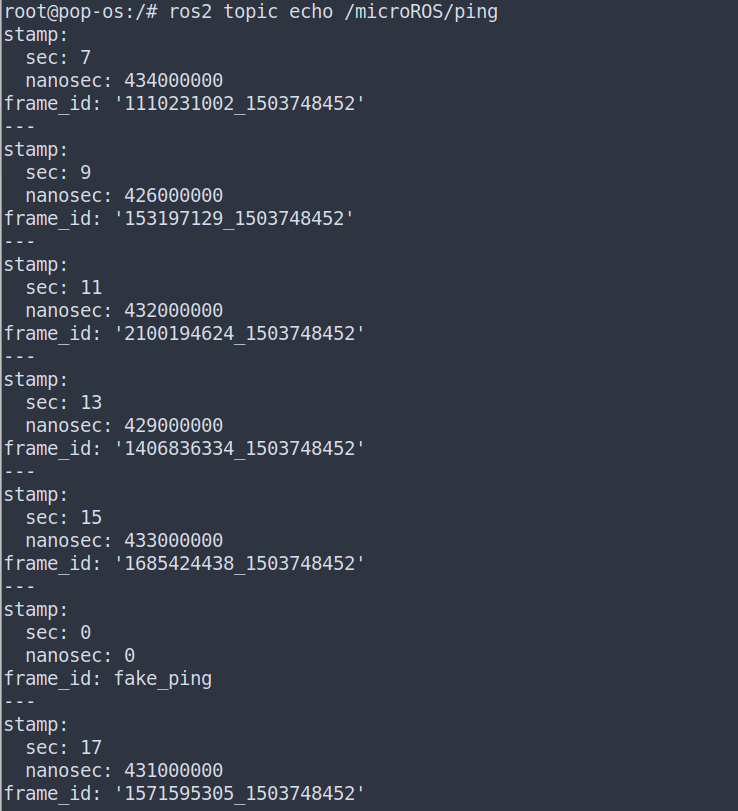
\includegraphics[width=.9\textwidth]{./img/pingpong.png}
  \caption{The ``fake ping'' pong return from the Nucleo board back to the Docker ROS2 instance, among it's normal pings.}
  \label{fig:pingpong}
\end{figure}


%--------------------------------------------------------------------------------------
\section{Blinking a LED (again)}
\label{sec:blinking-led-again}
As an extra proof that we correctly deployed the ``pingpong'' app on the Nucleo board, and in order to get used to modifying micro-ROS app, we made the pinging tasks also toggling LEDs on the board.\\

\subsection{Sources for the Nucleo's micro-ROS firmware}
\label{sec:sourc-nucl-micro}
A specific set of configuration files for our board is available at this \href{https://github.com/micro-ROS/micro_ros_setup/tree/humble/config/freertos/nucleo_f746zg}{GitHub link}.\\
However, this structure is really a general configuration for the building process for our board firmware. It turned out to be more useful to directly check the sources available that are use to build the apps.\\
This can be found inside the Docker, for what we are looking for: the code of the \verb|ping_pong| app:
\begin{tcolorbox}
\begin{verbatim}
./microros_ws/firmware/freertos_apps/apps/ping_pong/app.c
\end{verbatim}
\end{tcolorbox}

For other important files, we can note the path of the HAL library. This is crucial since this library is used by the STM32 boards to interact with the GPIO and needs to be loaded in your C code. Here is the path:
\begin{tcolorbox}
\begin{verbatim}
./microros/firmware/freertos_apps/microros_nucleo_\
f746zg_extensions/Drivers/STM32F7xx_HAL_Driver/\
Src/stm32f7xx_hal_gpio.c
\end{verbatim}
\end{tcolorbox}

\subsection{Modifying the firmware}
\label{sec:modifying-firmware}
The \href{https://gitlab.com/nucleo-144/documentation/-/blob/main/src/ping_pong.c}{C file} is available in this repository. It is a copy of the \verb|ping_pong| application C source and is to be modified to be able to drive some GPIOs.\\

Here are the key parts that were modified to be able to make it happen.\\

Firstly, we need the to include the HAL lib, as stated in the section \ref{sec:sourc-nucl-micro}:
\begin{tcolorbox}
\begin{verbatim}
#include "stm32f7xx_hal.h"
\end{verbatim}
\end{tcolorbox}

Since it is used later, we can setup this \verb|InitStruct| as a global static variable:
\begin{tcolorbox}
\begin{verbatim}
static GPIO_InitTypeDef  GPIO_InitStruct;
\end{verbatim}
\end{tcolorbox}

Then, going in the \verb|void appMain| function, we need to initialize and setup the HAL and GPIO setup:
\begin{tcolorbox}
\begin{verbatim}
HAL_Init();

__HAL_RCC_GPIOB_CLK_ENABLE();

GPIO_InitStruct.Mode  = GPIO_MODE_OUTPUT_PP;
GPIO_InitStruct.Pull  = GPIO_PULLUP;
GPIO_InitStruct.Speed = GPIO_SPEED_FREQ_VERY_HIGH;

GPIO_InitStruct.Pin = GPIO_PIN_0;
HAL_GPIO_Init(GPIOB, &GPIO_InitStruct);

GPIO_InitStruct.Pin = GPIO_PIN_7;
HAL_GPIO_Init(GPIOB, &GPIO_InitStruct);
\end{verbatim}
\end{tcolorbox}

Finally, we can call the \verb|Toggle| functions in the callback function for the ROS topics. In this case we are toggling the GPIO pin 0 (LD1) when a ping in send and the GPIO pin 7 (LD2) when a pong is sent (thus a ping is received).
It might also be interesting to send some status of the GPIO, which is what is done here in the \verb|sprintf| function.\\
The C below shows the two modifications for the \verb|void ping_timer_callback| function:
\begin{tcolorbox}
\begin{verbatim}
sprintf(outcoming_ping.frame_id.data,
     "Device ID: %d, GPIO: %d",
     device_id, HAL_GPIO_ReadPin(GPIOB, GPIO_PIN_0));
/* Toggles the LD1 when we ping */
HAL_GPIO_TogglePin(GPIOB, GPIO_PIN_0);
\end{verbatim}
\end{tcolorbox}


% --------------------------------------------------------------------------------------
\pagebreak
\section{Usage with N8M}
\label{sec:usage-with-n8m}
As the micro-ROS deployed system appear to work properly,it will become interesting
to make the board able to ``talk'' with my other Nitrogen8M ROS2 deployment.
This is a good exercise to see if everything works as expected, especially at
the DDS level.

\subsection{Deploying ROS2 on N8M}
\label{sec:deploying-ros2-n8m}
This step for having a clean installation of ROS2 on the Nitrogen8M board is detailed \href{https://gitlab.com/nitrogen8m/documentation/}{in my other guide about the board}, in the Section 5.

\subsection{Micro-ROS agent on the Nitrogen8M}
\label{sec:micro-ros-agent}
Once we have a ROS2 environment configured on our Nitrogen8M board, we need to install the tool for having the micro-ROS agent ready.
This requires a bit more work than in the docker example, since the one we have now is not prepared to build\footnote{Building the agent uses a lot of RAM, and the 2GB available on the board is not enough. A presented in the appendix \ref{appendix:adding-swap-part}, you should add and enable a swap partition.} run micro-ROS agent, thus more steps are needed, as seen next:
\begin{tcolorbox}
\begin{verbatim}
ROS_DISTRO=humble
source /opt/ros/$ROS_DISTRO/setup.bash

mkdir microros_ws
cd microros_ws
git clone -b $ROS_DISTRO \
    https://github.com/micro-ROS/micro_ros_setup.git \
    src/micro_ros_setup

sudo mkdir -p /etc/ros/rosdep/sources.list.d
wget https://raw.githubusercontent.com/ros/rosdistro/\
master/rosdep/sources.list.d/20-default.list

sudo apt update && rosdep update
rosdep install --from-paths src --ignore-src -y
sudo apt-get -y install python3-pip wget nano

colcon build
source ./install/local_setup.bash
ros2 run micro_ros_setup create_agent_ws.sh
ros2 run micro_ros_setup build_agent.sh
source ./install/local_setup.bash
ros2 run micro_ros_agent micro_ros_agent serial \
--dev /dev/ttyACM0
\end{verbatim}
\end{tcolorbox}

With the agent running (again, if the handshake for the topic being subscribed to does not happen, you should try to plug out and plug in back the Nucleo board(s) USB cable), you can now try to have the Nucleo boards communicating with the Cortex A53 running Linux and ROS2.\\

As usual, we can then open another terminal to the N8M board and run the following commands to echo the pings from the Nucleo board:
\begin{tcolorbox}
\begin{verbatim}
source /opt/ros/$ROS_DISTRO/setup.bash

ros2 topic echo /microROS/ping
\end{verbatim}
\end{tcolorbox}

If everything goes the right way, you should be able to see the pings from the board that are connected. If the LED modification was made, the blink should also happen, and if you have two Nucleo boards connected, they should be able to ping each other, blinking each other's ping and pong assigned LEDs. This is a proof of the resilience of the DDS setup, and a good way to see that everything works as expected.

% --------------------------------------------------------------------------------------
\section{Conclusion}
\label{sec:conclusion}
Now we were able to test a working micro-ROS - ROS2 environment, the next step will be to run micro-ROS on the Nitrogen8m core M4 and being able to communicated with the Linux side through shared memory.\\

These steps are core parts of my research project and will be discussed and presented in separated guides.


% --------------------------------------------------------------------------------------
\pagebreak
\appendix
\section{Nucleo filesystem from a container}
\label{appendix:nucl-filesyst-from}
It is possible to view the Nucleo board as a mountable volume by plugging in the \verb|USB PWR| port to your machine. The \verb|/dev/sdX| will be mounted as something similar to \verb|/media/user/NODE_F746ZG|.\\
It is also an option to mount this device from inside a Docker, for example with the following:
\begin{tcolorbox}
\begin{verbatim}
mkdir /tmp/nucleo
mount /dev/sda /tmp/nucleo
\end{verbatim}
\end{tcolorbox}

We can then upload the firmware to the board by moving the \verb|.bin| to the mounted volume:
\begin{tcolorbox}
\begin{verbatim}
cp firmware/freertos_apps/\
microros_nucleo_f746zg_extensions/build/micro-ROS.bin \
/tmp/nucleo/
\end{verbatim}
\end{tcolorbox}

However, this is not really needed, as the \verb|flash_firmware.sh| script provided for the board seems to work properly.

% --------------------------------------------------------------------------------------
\pagebreak
\section{Adding a swap partition}
\label{appendix:adding-swap-part}
This part is a copy from my \href{https://gitlab.com/nitrogen8m/documentation/}{own repository about the Nitrogen8M board}.\\

For this additional guide, and as stated previously, we will consider that the goal here is to use the NVMe SSD, with it's adapter, to have a swap partition. We also consider that the SSD is empty or that the data on it can be erased. If it is not the case, please backup your data somewhere else, for example by using a NFS volume.\\

Firstly, you'll need to delete the existing partition (if it exist), create the new partition, give it a size and assigning it the ``swap'' type.\\
In the example below, we are creating a 8GB swap partition on the \verb|/dev/nvme0n1|:
\begin{tcolorbox}
\begin{verbatim}
sudo fdisk /dev/nvme0n1
p
d
p
n
p
default
default
+8G
p
t
82
w
\end{verbatim}
\end{tcolorbox}

Then you can follow the next lines to state to Linux that the partition (in this case, the 2nd partition on the NVMe) is a swap, and finally setting up the \verb|fstab| so the swap can be started at boot. Reboot the device to test the whole setup:
\begin{tcolorbox}
\begin{verbatim}
sudo sync
sudo mkswap /dev/nvme0n1p2
sudo su -c 'echo "/dev/nvme0n1p2 swap swap defaults 0 0" \
>> /etc/fstab'
sudo reboot now
\end{verbatim}
\end{tcolorbox}

% --------------------------------------------------------------------------------------
\pagebreak

\section{STM32F4}
\label{appendix:stm32f4}
The figure \ref{fig:f4} below shows the two boards next to each other. The difference is usage are minimal and both were able to run the firmware almost the same way.

\begin{figure}[h]
  \centering
  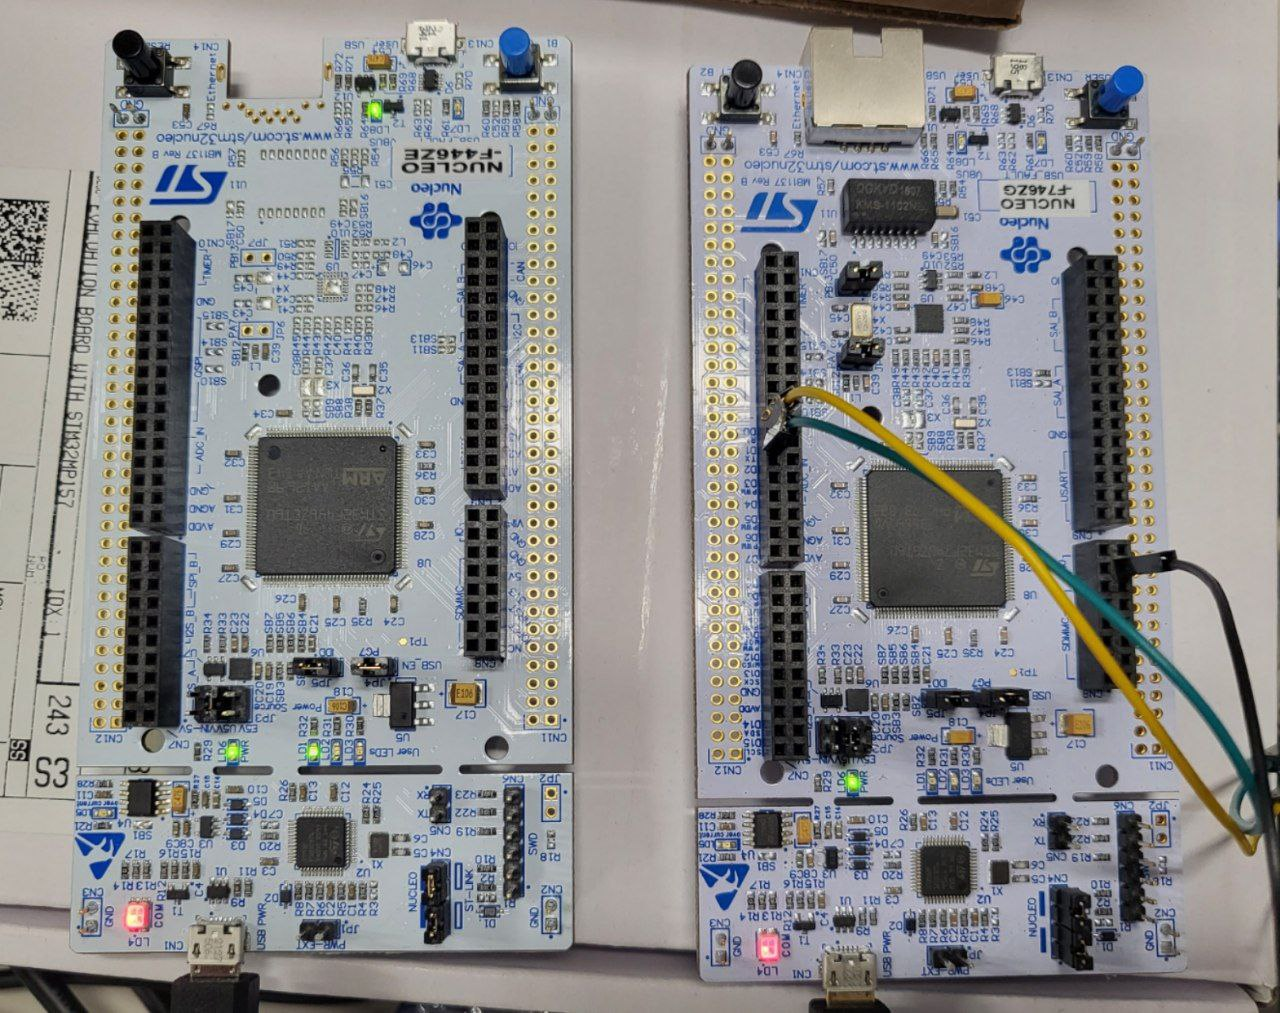
\includegraphics[width=.8\textwidth]{./img/f4.jpg}
  \caption{The STM32F4xx based board next to the F7xx used in this guide.}
  \label{fig:f4}
\end{figure}

There are only two minor differences that were encountered:
\begin{itemize}
\item By default the LED 1 on the F4 blinks, which is not the case on the F7 board.
\item When the ping-pong app was rebuilt to be able to blink LEDs, the name of the STM32 library to be included has t be changed: as presented in the section \ref{sec:modifying-firmware}, we need to include the \verb|stm32f7xx_hal.h|, but obviously for the F4 board, we must include \verb|stm32f4xx_hal.h| instead.
\end{itemize}


\end{document}